\selectlanguage{english}
\chapter{The Standard Model and beyond}
\label{Chapter1}
%SourceDoc tesi.tex

Particle Physics studies the building blocks of the matter, the so called fundamental particle, and how they are governed by the four fundamental forces\footnote{In the thesis, Natural Units will be used: $c=\hbar=1$,  where $\hbar=h/2\pi=6.58211889(26)\cdot10^{-23}MeV s$ and $c=299792458~ms^{-1}$.}. \\
The best theory, explaining our  understanding of these particles and forces, is the \textit{Standard Model} (SM): developed during the 1970s, it has successfully explained almost all experimental results and precisely predicted a wide variety of physical phenomena. \\
This chapter will describe in details the Standard Model and some theories developed in order to solve some unanswered questions.

\section{The Standard Model}
\label{cap1:SM}
\subsection{Fundamental Particles}
\label{cap1:pi}
All matter around us is made of elementary particles, the building blocks of matter. These particles are divided into two groups: \textit{leptons}, with an entire value of electric charge, and \textit{quarks}, with a fractional charge. Each group consists of six particles, which are related in pairs, or generations. The six quarks are paired in the three generations: the up quark and the down quark form the first generation, followed by the charm quark and strange quark, then the top quark and bottom (or beauty) quark.  The six leptons are similarly arranged in three generations: the electron and the electron neutrino, the muon and the muon neutrino, and the tau and the tau neutrino. While electron, muon and tau are charged particles, the neutrinos are electrically neutral. In table \ref{leptonsSM} and \ref{quarkSM}, the features of leptons and quarks.
\begin{table}[ht]	
	\begin{center}
		\begin{tabular}{|ccc|}
			\hline     & \textbf{Leptons} &   \\
			\hline   Flavor & Charge & Mass[MeV]  \\
			\hline
			\hline
			 neutrino e. ($\nu_{e}$) & 0 & $<0.002$   \\
			 electron ($e$) & -1 & 0.511   \\
			\hline
			 neutrino mu ($\nu_{\mu}$) & 0 & $<0.19$   \\
			 muon ($\mu$) & -1 & 105.66   \\
			\hline
			 neutrino tau ($\nu_{\tau}$) & 0 & $<18.2$ \\
			 tau ($\tau$) & -1 & 1776.86$\pm$0.12  \\
			\hline
			\hline
		\end{tabular}
	\end{center}
	\caption{Standard Model leptons features \cite{PDG}.}
	\label{leptonsSM}
\end{table}

\begin{table}[htbp]	
	\begin{center}
		\begin{tabular}{|ccc|}
			\hline    & \textbf{Quark} &   \\
			\hline   Flavor & Carica & Massa[GeV]  \\
			\hline
			\hline
			up (\emph{u}) & +2/3 & 0.0022$^{+0.0006}_{-0.0004}$ \\   
			down (\emph{d}) & -1/3 & 0.0047$^{+0.0005}_{-0.0004}$ \\
			\hline
			charm (\emph{c}) & +2/3 & $1.28\pm3$ \\
			strange (\emph{s}) & -1/3 & $0.096\pm0.084$ \\
			\hline
			top (\emph{t}) & +2/3 & $173.1\pm0.6$ \\
			bottom (\emph{b}) & -1/3 & 4.18$^{+0.04}_{-0.03}$ \\   
			\hline
			\hline
		\end{tabular}
	\end{center}
	\caption{Standard Model quarks features \cite{PDG}.}
	\label{quarkSM}
\end{table}

Beside these leptons and quarks, there are other particles responsible of carrying the fundamental forces, the so called \textit{bosons}. The Electromagnetic Force, responsible of all eletrical and magnetic phenomena, is mediated by the phtons {$\gamma$}; the Weak Force, responsible of some decays, is mediate by $W^{\pm}$ and $Z$ bosons; the Strong Force, responsible for example of the atomic structure, is mediated by the gluons ($g$). Last fundamental force, not yet included in the SM, is the Gravity that is the weakest. In table \ref{bosonsSM} the features of the bosons.
\begin{table}[htbp]	
	\begin{center}
		\begin{tabular}{|cccc|}
			\hline    Bosons & Interaction & Charge & Mass[GeV]  \\
			\hline
			\hline
			 photon ($\gamma$) &  Electromagnetic & 0 & 0   \\
			 \hline
			 $W^{\pm}$ & Weak & $\pm$1 & 80.385$\pm$0.015   \\
			 \hline 
             	 	 $Z^{0}$ & Weak & 0 & 91.1876$\pm$0.0021   \\
			 \hline
			 gluoni & Strong & 0 & 0 \\
			\hline
			\hline
		\end{tabular}
	\end{center}
	\caption{Standard Model bosons features \cite{PDG}.}
	\label{bosonsSM}
\end{table}


\subsection{Gauge Symmetries}
\label{cap1:gaugeSymm}
The present belief is that all particles interactions may be dictated by the so called \textit{local gauge symmetries} and this is connected with the idea that  the conserved physical quantities (such as electric charge) are conserved in local regions of space and not just globally\cite{HalzenMartin}. \\
%The connection between symmetries and conservation laws is best discussed in the framework of Lagrangian Field Theory.\\
The fundamental quantity in classical mechanics is the action \textit{S}, the time integral of the Lagrangian \textit{L}:
\begin{equation}
S = \int L\, dt = \int \mathcal{L}(\phi, \partial \phi / \partial x_{\mu}) \,d^{4}x
\end{equation}
where $\mathcal{L}$ is the Lagrangian Density\footnote{however, following standard use in field theory, we will often refer to $\mathcal{L}$ simply Lagrangian.}, 
and $\phi$ is the filed, itself a function of the continuous parameters $x_{\mu}$ \cite{Peskin}\cite{Maggiore}.
%\begin{equation}
%L \equiv T - V
%\end{equation}
%where T and V are the kinetic and potential energy of the system respectively.
The \textit{principle of least action} states that fixed the values of the coordinates at the initial time $t_{in}$ and at the final time $t_{f}$, then classical trajectory which satisfies these conditions is an extremum of the action. This leads to the \textit{Euler-Lagrange} equations (\ref{Eul_Lagr_Eq})
from which can be obtained the particle equations of motion.
\begin{equation}
\frac{\partial \mathcal{L}}{\partial \phi} - \frac{\partial}{\partial x_{\mu}}\frac{\partial \mathcal{L}}{\partial(\partial \phi / \partial x_{\mu})} = 0
\label{Eul_Lagr_Eq}
\end{equation}
%The relationship between symmetries and conservation laws is summarized in \textit{Noether's theorem}: 

\subsubsection{QED}\index{QED}\label{QED}
%Quantum electrodynamics (QED) describes the interactions between photons and electrons. 
The interaction of electron with photon is described by the Quantum Electrodynamics. 
Let's start with a complex field $\psi$ describing a free electron with mass m: its Lagrangian is
%Its motion is described by the Dirac Equation that follow from
% while the Dirac equation describes its motion. It can be shown Dirac equation follows from
\begin{equation}
\mathcal{L} = \bar{\psi}(i\gamma^{\mu}\partial_{\mu}-m)\psi
\label{L_electron}
\end{equation}
and its equation of motion can be deduced by the Dirac Equation, obtained substituting \ref{L_electron} in \ref{Eul_Lagr_Eq}. \\
The electromagnetic (em)  field instead is described by a four-vector $A_{\mu}$, the gauge potential. The field strength tensor is defined as:
\begin{equation}
F_{\mu\nu} = \partial_{\mu}A_{\nu} - \partial_{\nu}A_{\mu}
\label{F_em}
\end{equation}
and the equation of motion, in presence of an external current $J^{\mu}$ is:
\begin{equation}
\partial_{\mu}F^{\mu\nu} = QeJ^{\nu}
\label{Motion_em}
\end{equation}
In case now the electron interacts with the em field, the new Lagrangian is:
\begin{equation}
\mathcal{L}_{EM} = \bar{\psi}(i\gamma^{\mu}D_{\mu}-m)\psi - \frac{1}{4}F_{\mu\nu}F^{\mu\nu}
\label{L_electron_em}
\end{equation}
where $D_{\mu}$, known as covariant derivative, is defined as
\begin{equation}
D_{\mu} = \partial_{\mu} + ieQA_{\mu}
\label{D_covariante}
\end{equation}
and the last term in \ref{L_electron_em} stands for Maxwell's equation. \\
It can be shown that \ref{L_electron_em} is invariant under the phase transformation:
\begin{equation}
\psi(x)\to e^{-iQ\theta} \psi(x)
\label{global_trans}
\end{equation}
with $\theta \in \Re$. This transformation belongs to the group U(1) and according to Noether's theorem, it implies the existence of a conserved current: the electric charge.
In this case, known as \textit{global "gauge" invariance}, once the value of $\theta$ is fixed, it is specified for all space and time. \\
More interesting is the case in which the parameter $\theta$ depends on space and time in a completely arbitrary way:
\begin{equation}
\psi(x)\to e^{-iQ\theta(x)} \psi(x)
\label{local_trans}
\end{equation}
and the Lagrangian \ref{L_electron_em} is not invariant.
It can be shown that, in oder to restore the Lagrangian invariance, the potential $A_{\mu}$ must satisfy following condition:
\begin{equation}
A_{\mu} \to A_{\mu} + \frac{1}{e}\partial_{\mu}\theta
\label{A_trans}
\end{equation}
Under \ref{local_trans} and \ref{A_trans} the Lagrangian \ref{L_electron_em} is invariant.\\ 
One can observe the absent of mass term in the Lagrangian: this means that the boson associated to the potential $A_{\mu}$, the photon, must be massless: the presence of a mass term would make the Lagrangian not invariant under gauge transformation. \\

\subsubsection{QCD}\index{QCD}\label{QCD}
The interaction between quarks and gluons is described by the Quantum Chromodynamics. \\
For quarks \cite{QCD}, it must be considered a new quantum number, the colour, such that each species of quark may have three different colours: $q_{j},\ j = 1, 2, 3$ (red, green, blue). In order to avoid the existence of non-observed extra states with non-zero colour, one needs to further postulate that all asymptotic states are colourless, i.e. singlets under rotations in colour space. This assumption is known as the confinement hypothesis, because it implies the non-observability of free quarks: since quarks carry colour they are confined within colour-singlet bound states. \\
For free quark described by the field $q_{j}$, the Lagrangian is:
\begin{equation}
\mathcal{L} = \bar{q_{j}}(i\gamma^{\mu}\partial_{\mu} - m)q_{j}
\label{L_quark}
\end{equation}
In order to describe the  interaction between quarks and gluons, it is needed to change the quark derivative by covariant objects. Since there are now eight independent gauge parameters, eight different gauge bosons $G^{\mu}_{a}(x)$, the so-called gluons, are needed:
\begin{equation}
D^{\mu}_{q_{f}} \equiv [\partial^{\mu}- ig_{s}\frac{\lambda^{a}}{2}G^{\mu}_{a}(x)]
\label{D_covariante_qcd}
\end{equation}
The corresponding field strengths are also introduced:
\begin{equation}
G^{\mu\nu}_{a} = \partial^{\mu}G^{\nu}_{a} - \partial^{\nu}G^{\mu}_{a} + g_{s}f^{abc}G^{\mu}_{b}G^{\nu}_{c}
\label{G_munu}
\end{equation}
where $g_{s}$ is the constant coupling.
Hence, in case of interaction the new Lagrangian is:
\begin{equation}
\mathcal{L}_{QCD} = \bar{q_{j}}(i\gamma^{\mu}D_{\mu} - m)q_{j} -\frac{1}{4}G^{\mu\nu}_{a}G^{a}_{\mu\nu}
\label{L_quark_gluon}
\end{equation}
It can be shown \ref{L_quark_gluon} in invariant under arbitrary global $SU(3)_{C}$ transformations in colour space \ref{q_tranf_global}:
\begin{equation}
q(x) \to q'(x) = Uq(x) \equiv e^{i\theta_{a}T^{a}}q(x), \quad a = 1, 2, ...,8
\label{q_tranf_global}
\end{equation}
where $T_{a}$ are the generators of the SU(3) (n = $N^{2} - 1 = 3^{2} - 1 = 8)$ group linked with the $\lambda_{a}$ Gell-Mann matrices. \\
More interesting is the case in which $\theta$ depends on local coordinates, $\theta_{a}$ = $\theta_{a}$(x):
\begin{equation}
q(x) \to q'(x) = Uq(x) \equiv e^{i\theta_{a}(x)\frac{\lambda^{a}}{2}}q(x), \quad a = 1, 2, ...,8
\label{q_tranf_local}
\end{equation}
The group is non-Abelian since not all the generators $\lambda_{a}$ commute with each other. \\
To ensure the invariance of the Lagrangian \ref{L_quark_gluon}, the gauge fields must transform as follow:
\begin{equation}
G^{a}_{\mu} \to G^{a}_{\mu} - \frac{1}{g_{s}} \partial_{\mu}\theta_{a} - f_{abc}\theta^{b}G^{c}_{\mu}
\label{G_tranf_local}
\end{equation}
The field tensor $G^{\mu\nu}_{a}$ has a remarkable new property: imposing gauge symmetry (\ref{q_tranf_local} and \ref{G_tranf_local}) has required that the kinematic energy term in \ref{L_quark_gluon} in not purely kinetic but includes an induced self-interaction between the gauge bosons. Decomposing the Lagrangian into its different pieces, there are three terms analogues to QED describing the free propagation of quarks and gluons and the quark-gluon interaction. The remaining two terms show the presence of three and four gluon self-coupling in QCD and reflect the fact that gluons themselves carry color charge. They have no analogue in QED and arise on account of the non-Abelian character of the gauge group. As in QED, the absence of a mass term implies gluons must be massless.\\

\subsubsection{The electroweak theory}\index{EWK}
Low-energy experiments have provided a large amount of information about the dynamics underlying flavour-changing processes. The detailed analysis of the energy and angular distributions in $\beta$ decays, such as $\mu^{-} \to e^{-}\bar{\nu}_{e}\nu_{\mu}$, made clear that only the left-handed (right-handed) fermion (antifermion) chiralities participate in those weak transitions. Moreover, the strength of the interaction appears to be universal. \\
Using gauge invariance, it is possible to determine the right QED (\ref{QED} and QCD \ref{QCD} Lagrangians. To describe weak interactions, a more elaborated structure is needed, with several fermionic flavours and different properties for left- and right-handed fields. Moreover, the left-handed fermions should appear in doublets, and we would like to have gauge bosons in addition to the photon. The simplest group with doublet representations is SU(2) while to include also the electromagnetic interactions an additional U(1) group is needed. The obvious symmetry group to consider is then:
\begin{equation}
G \equiv SU(2)_{L} \otimes U(1)_{Y}
\label{EWK_group}
\end{equation}
where L refers to left-handed fields and Y stands for the weak hypercharge. \\
Let's consider a single family of leptons:
\begin{equation}
%\chi_L	&= \begin{pmatrix}\nu_{\emph{l}} \\\emph{l}^-\end{pmatrix}_L
\chi_{L} =  {\nu_{l} \choose l^{-}}_{L}, \quad \psi_{R} = l^{-}_{R}
\label{EWK_Singlet_doublet_Leptons}
\end{equation}
or for quarks
\begin{equation}
%\chi_L	&= \begin{pmatrix}\nu_{\emph{l}} \\\emph{l}^-\end{pmatrix}_L
\chi_{L} =  {u \choose d}_{L} , \quad \psi_{R} = u_{R},\ or\ d_{R}
\label{EWK_Singlet_doublet_Leptons}
\end{equation}
As in QED and QCD case, starts with free Lagrangian:
\begin{equation}
\mathcal{L} = i\bar{\chi}_{L}\gamma^{\mu}\partial_{\mu}\chi_{L} + i\bar{\psi}_{R}\gamma^{\mu}\partial_{\mu}\psi_{R}
\label{L0_EWK}
\end{equation}
The interaction is again introduced changing the derivative with the covariante:
\begin{equation}
D_{\mu} = \partial_{\mu} + igW_{\mu}^{a}T^{a} + ig'B_{\mu}Y
\label{D_EWK}
\end{equation}
where $W_{\mu}^{a}$ a = 1, 2, 3 are the three gauge bosons associated with the group $SU(2)_{L}$, $T^{a}$ its generators and g the constant couplings; $B_{\mu}$, Y and g are instead respectively the gauge boson, the generator and the constant coupling for the group $U(1)_{Y}$.
With $W_{\mu}^{a}$ and $B_{\mu}$ can be introduced also the tensor strength fields:
\begin{equation}
\begin{split}
W^{\mu\nu}_{a} &= \partial^{\mu}W^{\nu}_{a} - \partial^{\nu}W^{\mu}_{a} + g\epsilon^{abc}W^{\mu}_{b}W^{\nu}_{c} \\
B^{\mu\nu} 	 &= \partial^{\mu}B^{\nu} - \partial^{\nu}B^{\mu}
\label{WB_munu}
\end{split}
\end{equation}
Therefore, the properly Lagrangian is given by:
\begin{equation}
\mathcal{L} = i\bar{\chi}_{L}\gamma^{\mu}D_{\mu}\chi_{L} + i\bar{\psi}_{R}\gamma^{\mu}D_{\mu}\psi_{R} - \frac{1}{4}B_{\mu\nu}B^{\mu\nu} - \frac{1}{4}W_{\mu\nu}W^{\mu\nu}
\label{L_EWK}
\end{equation}
In \ref{L_EWK} $W_{\mu\nu} = W^{a}_{\mu\nu}\sigma^{a}/2$ with $\sigma^{a}$ 2x2 Pauli's matries. \\
As in QED and QCD case, also electroweak interaction is invariant under global transformation:
\begin{equation}
\begin{split}
\chi_{L} \to \chi_{L}' &= e^{i\alpha_{a} T^{a}  + i\beta Y} \chi_{L} \\
\psi_{R} \to \psi_{R}' &= e^{i\beta Y} \psi_{R} \\
\label{EWK_global}
\end{split}
\end{equation}
Moving to local transformation, in order to guarantee Lagrangian \ref{L_EWK} to be invariant, the gauge bosons must have following transformation rules:
\begin{equation}
\begin{split}
W^{a}_{\mu} &\to U_{L}(x) W^{a}_{\mu} \frac{\sigma_{a}}{2} U_{L}(x)^{\dagger} - \frac{i}{g}\partial_{\mu}U_{L}(x) U_{L}(x)^{\dagger}, \\
B_{\mu} &\to B_{\mu} + \frac{1}{g'}\partial_{\mu}\beta
\label{EWK_global}
\end{split}
\end{equation}
where $U(x)_{L} = e^{i\sigma_{a} / 2\ \alpha(x)^{a}}$. The transformation of $B_{\mu}$ is identical to the one obtained in QED for the photon, while the $SU(2)_{L}\ W^{a}_{\mu}$ fields transform in analogous way to the gluon fields of QCD. \\
The gauge symmetry forbids to write a mass term for the gauge bosons in \ref{L_EWK}. Fermionic masses are also not possible, because they would communicate the left- and right-handed fields, which have different transformation properties, and therefore would produce an explicit breaking of the gauge symmetry. Thus, the $SU(2)_{L} \otimes U(1)_{Y}$ Lagrangian in \ref{L_EWK} only contains massless fields.\\
The term containing the $SU(2)_{L}$ matrix:
\begin{equation}
\frac{\sigma^{a}}{2}W_{\mu}^{a} = \frac{1}{\sqrt{2}}\begin{pmatrix} \sqrt{2}W^{3}_{\mu} & W_{\mu}^{+} \\ W_{\mu}^{-} & - \sqrt{2}W^{3}_{\mu} \end{pmatrix}
\end{equation}
gives rise to charged-current interactions with the bosons field $W_{\mu}^{\pm} \equiv (W^{1}_{\mu} \mp iW^{2}_{\mu}) / \sqrt{2}$. \\
La Lagrangian \ref{L_EWK}  contains also interactions with the neutral gauge field $W^{3}_{\mu}$ and $B_{\mu}$; one can define
\begin{equation}
Z_{\mu} = \frac{gW^{3}_{\mu} - g'B_{\mu}}	{\sqrt{g^{2}+g'{2}}}, \quad A_{\mu} = \frac{gW^{3}_{\mu} + g'B_{\mu}}	{\sqrt{g^{2}+g'{2}}}
\label{A_Z}
\end{equation}
and thinking them as a rotation, introducing the Weinberg angle $\theta_{W}$ so that $\cos\theta_{W} = g/{\sqrt{g^{2}+g'{2}}}$ (and $\sin\theta_{W} = g'/{\sqrt{g^{2}+g'{2}}}$):
\begin{equation}
Z_{\mu} = \cos\theta_{W}W^{3}_{\mu} - \sin\theta_{W}B_{\mu}, \quad A_{\mu} = \sin\theta_{W}W^{3}_{\mu} + \cos\theta_{W}B_{\mu}
\label{A_Z_2}
\end{equation}
or reversing:
\begin{equation}
{W^{3}_{\mu} \choose B_{\mu}} \equiv \begin{pmatrix} \cos\theta_{W} & \sin\theta_{W} \\ -\sin\theta_{W} & \cos\theta_{W} \end{pmatrix} {Z_{\mu} \choose A_{\mu}}
\label{W_B_A_Z}
\end{equation}
With these definitions, it can be observed the $A_{\mu}$ in\ref{L_EWK} couple in the same way with $l_{L}$ and $l_{R}$ as the photon: to get QED from these one needs to impose
\begin{equation}
g\sin\theta_{W} = g'\cos\theta_{W} = e
\label{g_gprime}
\end{equation}
At the same time, $Z_{\mu}$, can be identify with the Z boson, mediator of the Weak Interaction. \\
Once again, no mass term is present in \ref{L_EWK} and this means that $W^{\pm}$ and Z must be massless: this is in contrast with experimental evidence \cite{Wboson}\cite{Zboson}. \\
The way to generate the mass of the particle is through the so called \textit{Spontaneous Symmetry Breaking} (SSB): this mechanism appear in those cases where one has a symmetric Lagrangian, but a non-symmetric vacuum. 

\subsection{Spontaneous Symmetry Breaking and the Higgs Boson}
Let's consider a complex scalar field $\phi(x) = (\phi_{1} + \phi_{2}) / \sqrt{2}$, with Lagrangian:
\begin{equation}
\mathcal{L} \equiv T - V = (\partial_{\mu}\phi)^{*}(\partial^{\mu}\phi) - \mu^{2}(\phi^{*}\phi)-\lambda(\phi^{*}\phi)^{2}
\label{L0}
\end{equation}
\ref{L0} is invariant under global phase transformation of the scalar field (it possesses a U(1) global gauge symmetry). \\
Considering the case when $\lambda > 0$, for the quadratic piece there are two possibilities:
\begin{itemize}
\item{$\mu^{2} > 0$:} the potential has only the trivial minimum $\phi = 0$
\item{$\mu^{2} < 0$:} the minimum is every point belong to the circle (in the $\phi_{1}, \phi_{2}$) of radius $\nu$ such that:
	\begin{equation}
	(\phi_{1})^{2}+(\phi_{2})^{2} = \nu^{2} \quad with\ \nu^{2} = - \frac{\mu^{2}}{\lambda}
	\end{equation}
	as shown in \figurename~\ref{V_phi_potential}
\end{itemize}
\begin{figure}[htbp]
\centering
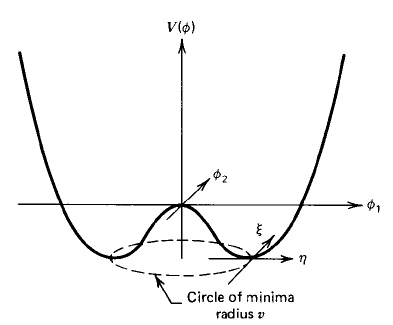
\includegraphics[width=0.45\textwidth]{Images/Vphi.png}
\caption{The potential $V(\phi)$ for a complex scalar field with $\lambda > 0$ and $\mu^{2} < 0$. }
\label{V_phi_potential}
\end{figure}
Owing to the U(1) phase-invariance of the Lagrangian \ref{L0}, there is an infinite number of degenerate states of minimum energy. 
By choosing a particular solution, $\phi_{1} = \nu$ and $\phi_{2} = 0$, as the ground state, the symmetry gets spontaneously broken. Parametrising the excitations over the ground state as:
\begin{equation}
\phi(x) \equiv \frac{1}{\sqrt{2}}[\nu+\eta(x)+i\xi(x)]
\label{phi_expansion}
\end{equation}
and substituting into \ref{L0}, one obtains:
\begin{equation}
\mathcal{L'} = \frac{1}{2}(\partial_{\mu}\xi)^{2} + \frac{1}{2}(\partial_{\mu}\eta)^{2} + \mu^{2}\eta^{2} + const. + O(\eta^{3})+O(\xi^{3})
\label{L0_prime}
\end{equation}
The third term has the form of a mass term for $\eta$-field: the $\eta$-mass is $m_{\eta} = \sqrt{-2\mu^{2}}$. The first term in \ref{L0_prime} represents the kinetic energy of the $\xi$-field but there is no corresponding mass term for the $\xi$. The fact there are massless excitations associated with the SSB mechanism is completely general result, known as the \textit{Goldstone theorem}: if a Lagrangian is invariant under a continuous symmetry group G, but the vacuum is only invariant under a subgroup $H\subset G$, then there must exist as many massless spin-0 particles (Goldstone bosons) as broken generators (i.e., generators of G which do not belong to H).
\subsubsection{The Higgs Mechanism: U(1) local gauge symmetry}
Let's move to consider the case for spontaneous breaking of U(1) local gauge symmetry.\\
Taking into account the covariant derivative \ref{D_covariante} where the gauge filed transforms as in \ref{A_trans}, the new Lagrangian can be written as
\begin{equation}
\mathcal{L} = D^{\mu}\phi^{*}D_{\mu}\phi -\mu^{2}\phi^{*}\phi-\lambda(\phi^{*}\phi)^{2}-\frac{1}{4}F_{\mu\nu}F^{\mu\nu}
\label{L0_U1}
\end{equation}
If $\mu^{2} > 0$, \ref{L0_U1} is just the QED Lagrangian for a charged scalar particle of mass $\mu$.
For the case $\mu^{2} < 0$, it is interesting to note that to lowest oder in $\xi$, \ref{phi_expansion} can be expressed as
\begin{equation}
\phi(x) \equiv \frac{1}{\sqrt{2}}[\nu+\eta(x)]e^{i\xi(x)/\nu}
\label{phi_expansion_2}
\end{equation}
and this suggests to use different set of real field: h, $\theta$, $A_{\mu}$ where now
\begin{equation}
\begin{split}
\phi(x) &\to \frac{1}{\sqrt{2}}[\nu+h(x)]e^{i\theta(x)/\nu}, \\
A_{\mu} &\to A_{\mu}+ \frac{1}{e\nu}\partial_{\mu}\theta
\end{split}
\label{new_phi_A}
\end{equation}
This is a particular choice of gauge, with $\theta(x)$ chosen so that h is real. Substituting \ref{new_phi_A} in \ref{L0_U1}, one obtains:
\begin{equation}
\begin{split}
\mathcal{L}' = &\frac{1}{2}(\partial_{\mu}h)^{2}-\lambda\nu^{2}h^{2}+\frac{1}{2}e^{2}\nu^{2}A_{\mu}^{2}-\lambda\nu h^{3}-\frac{1}{4}\lambda h^{4}\\
&+\frac{1}{2}e^{2}A_{\mu}^{2}h^{2}+\nu e^{2}A_{\mu}^{2}h-\frac{1}{4}F_{\mu\nu}F^{\mu\nu}
\end{split}
\label{L0_U1_prime}
\end{equation}
The Goldstone boson does not appear in the theory. That is because it corresponding only to the freedom to make a gauge transformation. The Lagrangian \ref{L0_U1_prime} describes just two interacting massive particles, a vector gauge bosoon $A_{\mu}$ and a massive scalar h, which is called a \textit{Higgs particle}. This is called the "\textit{Higgs mechanism}".\\
%\subsubsection{The Higgs Mechanism for $SU(2)_{L} \otimes U(1)_{Y}$ symmetry
Consider now the case of  $SU(2)_{L} \otimes U(1)_{Y}$ symmetry.
The Lagrangian
\begin{equation}
\mathcal{L} = (\partial_{\mu}\phi)^{\dagger}(\partial^{\mu}\phi)-\mu^{2}\phi^{\dagger}\phi-\lambda(\phi^{\dagger}\phi)^{2}
\label{L0_SU2}
\end{equation}
where $\phi$ is an SU(2) doublet of complex scalar fields:
\begin{equation}
\phi = {\phi_{\alpha} \choose \phi_{\beta}} = \frac{1}{\sqrt{2}}{\phi_{1}+i\phi_{2} \choose \phi_{3}+i\phi_{4}}
\label{phi_SU2}
\end{equation}

%Replacing the covariant derivative \ref{D_covariante} where 








\begin{comment}
Consider a simple case of a Lagrangian describing a scalar particle:
\begin{equation}
\mathcal{L} \equiv T - V = \frac{1}{2}(\partial \phi)^{2}-(\frac{1}{2}\mu^{2}\phi^{2} + \frac{1}{4}\lambda\phi^{4})
\label{L0}
\end{equation}
with $\lambda > 0$; keeping the first two allowed terms in the general expansion of V in power of $\phi$ guarantee \ref{L0} to be invariant under the symmetry operation $\phi \to -\phi$. 
The two possible form of the potential are shown in \figurename~\ref{V_phi_potential}
\begin{figure}[htbp]
\centering
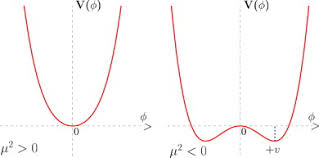
\includegraphics[width=0.45\textwidth]{Images/V_phi_potential}
\caption{The potential $V(\phi) = \frac{1}{2}\mu^{2}\phi^{2} + \frac{1}{4}\lambda\phi^{4}$ for (a) $\mu^{2} > 0$ and (b) $\mu^{2} < 0$.  \textbf{CAMBIA IMMAGINE: FA SCHIFO}}
\label{V_phi_potential}
\end{figure}
In the case $\mu^{2}$ is positive, the ground state (the vacuum) correspond to $\phi = 0$ and obeys the reflection symmetry of the Lagrangian. More interesting is the case in which $\mu^{2}$ is negative and the potential has two minima:
\begin{equation}
\phi = \pm\nu \quad\ with\ \nu = \sqrt{-\mu^{2}/\lambda}
\end{equation}
Perturbative calculations should involve expansions around the classical minimum\footnote{choosing $\phi = \nu$ does not imply any loss of generality since $\phi = -\nu$ can always be reached by reflection symmetry.}:
\begin{equation}
\phi(x) = \nu + \eta(x)
\label{phi_perturbative}
\end{equation}

\end{comment}
